% !TeX spellcheck = en_US
\documentclass[a4paper,twocolumn]{article}

\usepackage{fullpage}
\usepackage{fourier}
\usepackage{amsmath}
\usepackage{xcolor}
\usepackage{graphicx}
\usepackage{titlesec}
\usepackage{hyperref}
\usepackage{cleveref}
\usepackage{tabularx}
\usepackage{todonotes}
\usepackage{verbatim}
\usepackage[T1]{fontenc}
\usepackage[utf8]{inputenc}

%\titleformat{\subsection}[hang]{\large\bfseries}{\alph{subsection})\quad}{0pt}{}

\newcommand{\twodo}{\vspace{11pt}\textcolor{red}{\textbf{todo}}}
\newcommand{\subtask}[2]{\paragraph{#1)} \textit{#2} \newline}

\title{\textbf{Exercises for Image Processing 1}\\Problem Sheet 5}
\author{Axel Brand\\6145101 \and Nourhan Elfaramawy\\6517858 \and Sibel Toprak\\6712316}

\begin{document}
	\maketitle
	
	\section{Theoretical Problems}
	
	\subsection{(Lossless) Image Compression}
	
	\paragraph{a)} % What is the entropy of such documents?
	The \textit{entropy} of such documents can be computed using the following formula:
	\begin{align*}
	H = \sum_{g=0}^{G-1} P(g) \cdot \log_{2}\left(\frac{1}{P(g)}\right)
	\end{align*}
	Here, $G$ is the number of colors and $P(g)$ is the probability with which a particular color $g$ occurs in such a document. The following are the colors and their respective probabilities:
	\begin{center}
		\begin{tabular}{l r}
			$\mathbf{g}$ & $\mathbf{P(g)}$ \\
			\hline
			White  & 0.9   \\
			Black  & 0.08  \\
			Blue   & 0.012 \\
			Red    & 0.005 \\
			Green  & 0.002 \\
			Yellow & 0.001 \\
		\end{tabular}
	\end{center}
	Given these, we obtain the following intermediate results as well as the overall result for the entropy:
	\begin{align*}
	H
	&= 0.9 \cdot \log_{2}\left(\frac{1}{0.9}\right)
	&(\approx 0.13680) \\
	&+ 0.08 \cdot \log_{2}\left(\frac{1}{0.08}\right)
	&(\approx 0.29151) \\
	&+ 0.012 \cdot \log_{2}\left(\frac{1}{0.012}\right)
	&(\approx 0.07657) \\
	&+ 0.005 \cdot \log_{2}\left(\frac{1}{0.005}\right)
	&(\approx 0.03822) \\
	&+ 0.002 \cdot \log_{2}\left(\frac{1}{0.002}\right)
	&(\approx 0.01793) \\
	&+ 0.001 \cdot \log_{2}\left(\frac{1}{0.001}\right)
	&(\approx 0.00997) \\
	&\approx 0.570998
	\end{align*}
	
	Basically, the calculated value tells how much information is contained in these documents. One can say that the more unpredictable the color of the pixels in the document is, the more information the overall document will contain. For the statistics given above however, it is to be expected that the entropy value is pretty low: There is low uncertainty as to what color a pixel will be, with a 90\% probability of it being white, yielding this low of a value for the entropy. If all colors were approximately equally probable on the other hand, the entropy would be somewhat equal to the number of bits required for coding.\footnote{\url{https://simple.wikipedia.org/wiki/Information_entropy}}
	
	\begin{comment}
		Very intuitive example from "Simple Wikipedia":
		
		Let's look at an example. If someone is told something they already know, the information they get is very small. It will be pointless for them to be told something they already know. This information would have very low entropy.
		
		If they were told about something they knew little about, they would get much new information. This information would be very valuable to them. They would learn something. This information would have high entropy.
	\end{comment}
	
	\paragraph{b)} % Design a Huffman code for the pixels.
	See \Cref{fig:huffman_code} for the resulting Huffman code.
	\begin{figure*}[t]
		\begin{minipage}{0.5\textwidth}
			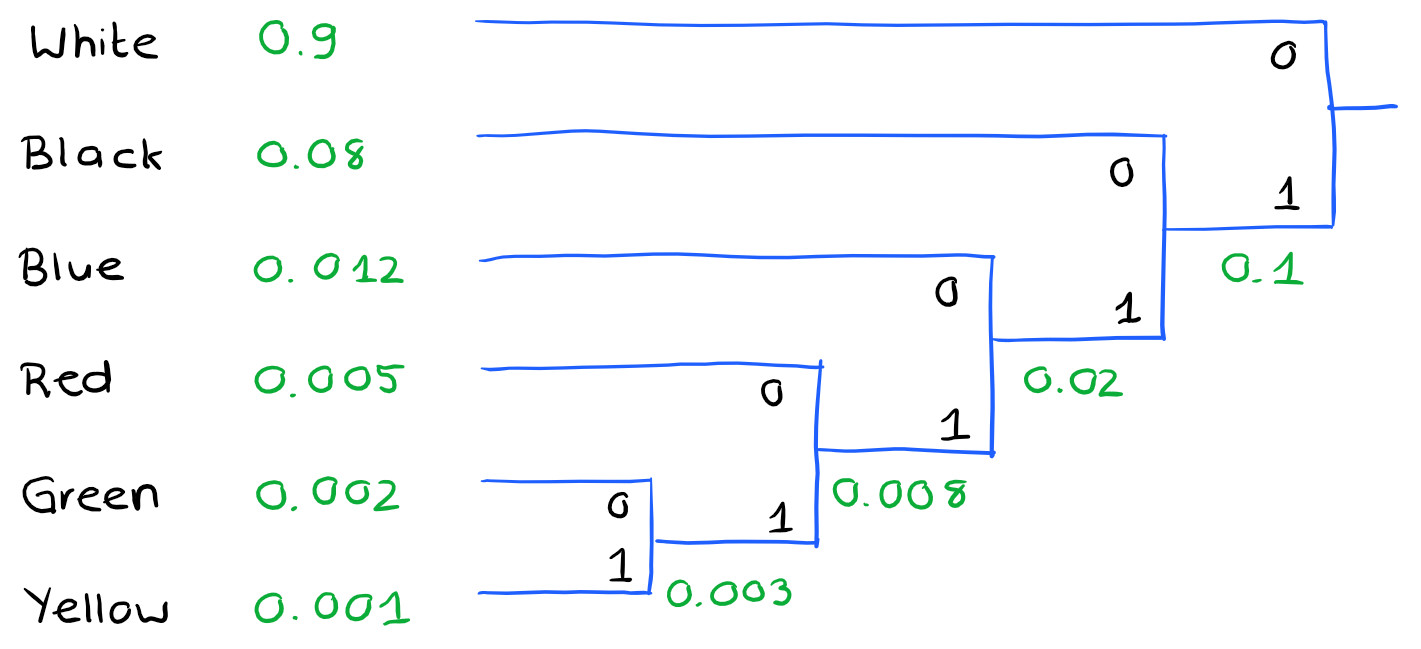
\includegraphics[width=\linewidth]{figures/huffman_code.png}
		\end{minipage}
		\hfill
		\begin{minipage}{0.4\textwidth}
			\begin{tabular}{l r r c}
				\textbf{Color} & \textbf{Probability} & \textbf{Code} & \textbf{Length}\\
				\hline
				White & 0.9 & 0 & 1 \\
				Black & 0.08 & 10 & 2 \\
				Blue & 0.012 & 110 & 3 \\
				Red & 0.005 & 1110 & 4 \\
				Green & 0.002 & 11110 & 5 \\
				Yellow & 0.001 & 11111 & 5
			\end{tabular}
		\end{minipage}
		\caption{\textit{Left:} Applying the Huffman coding scheme to create variable-length codes with minimal average code word length for the colors. \textit{Right:} The resulting color code words and their lengths.}
		\label{fig:huffman_code}
	\end{figure*}
	
	\paragraph{c)} % What is the mean length of a code word?
	The \textit{mean length of a code word} can be computed by weighting the length of the Huffman codes obtained for each color with the respective probabilities and summing them up:
	\begin{align*}
	\text{mean} 
	&= 0.9 \cdot 1 	 &(=0.9) \\
	&+ 0.08 \cdot 2  &(=0.16) \\
	&+ 0.012 \cdot 3 &(=0.036) \\ 
	&+ 0.005 \cdot 4 &(=0.02) \\ 
	&+ 0.002 \cdot 5 &(=0.01) \\ 
	&+ 0.001 \cdot 5 &(=0.005) \\ 
	&= 1.131
	\end{align*}
	See \Cref{fig:huffman_code} for the values.
	
	\paragraph{d)} % What is the redundancy of the following 4-bit code?
	The redundancy $r$ of the given 4-bit code can be computed like so:
	\begin{align*}
	r = b - H
	\end{align*}
	Here, $b$ is the number of bits used for each pixel, which is four in this case, and $H$ is the entropy of the pixel source, which we computed above already. Thus, we obtain:
	\begin{align*}
		r = 4 - 0.570998 = 3.429002
	\end{align*}
	
	\subsection{Image Segmentation}
	
	\paragraph{a)} % When may simple threshold-based segmentation approaches be applicable for image segmentation, when not? Give at least one example for each.
	Threshold-based segmentation approaches can be applicable for image segmentation, only if the image has contrast between the whole object we want to segment and the background in uniform illumination conditions. For example, see Fig. 1 & 2 below.
	
	
	\paragraph{b)} % Does the bi-modality of the image histogram guarantee successful image segmentation if threshold-based image segmentation is applied and the threshold is selected in the minimum between the two histogram maxima?
	No, because the bi-modality of the histogram indicates that the image has two areas with high contrast, but does not guarantee that we can segment the object from the background in an image. For example, if the image has non-uniform illumination conditions, it is not possible to segment the object in the image based on a unique threshold, because the threshold-based segmentation relies only on the distribution of the intensity values of the image and not on its spatial properties, such as edge-detection.
	
	\paragraph{c)} % Explain the need of component labeling for object detection after thresholding.
	
	The need of component labeling for object detection after thresholding is due to the classification/distinguishment of pixels in each region of the image.
	
	\paragraph{d)} % What is the most typical problem in edge detection approaches? How does the Canny-algorithm try to enhance the segmentation quality?

	The most common problem in edge detection aaproaches is its sensitvity to noise, which makes edge detection inaccurate.
	
	Canny-Algorithm:
	What Canny-algorithm does is that it takes the sobel operator and use is to thin the orientation of the edge, and then use the thresholding to find dominant edges in the image.
	The optimality of canny edge detection consists of the following criterion:
	1) The detection, which indicates all the important edges should not be missed.
	2) The localization, which minimizes the distance between the actual and the located position of the egdes.
	3) The one response, which minimizes multiple reponses to a single edge. Hence, reduces noise.
	
	
	\section{Practical Problems}
	
	\subsection{(Lossy) Image Compression}
	
	\paragraph{a)} See file \texttt{task\_2\_1.py} for the computation.
	
	\paragraph{b)} % What is the mean quadratic error (MSE) for x_1' when it is reconstructed using A_3^T?
	The Karhunen-Loève compression technique can, for instance, be used to code $2 \times 2$ images with pixels $x_1, x_2, x_3$ and $x_4$ with 3 values, namely $y_1, y_2$ and $y_3$, by means of the transform matrix $A_3$:
	\begin{align*}
	\begin{bmatrix}
	y_1 \\ y_2 \\ y_3
	\end{bmatrix}
	= A_3 \cdot 
	\begin{bmatrix}
	x_1 \\ x_2 \\ x_3 \\ x_4
	\end{bmatrix}
	\end{align*}
	This is done in a way that the original image can easily be reconstructed from the compressed values with minimal error with the help of the very same, but now transposed, transform matrix $A_3$:
	\begin{align*}
	\begin{bmatrix}
	x_1^{\prime} \\ x_2^{\prime} \\ x_3^{\prime} \\ x_4^{\prime}
	\end{bmatrix}
	= A_3^T \cdot
	\begin{bmatrix}
	y_1 \\ y_2 \\ y_3
	\end{bmatrix}
	\end{align*}
	Because this compression is lossy, the original image will not be reconstructed perfectly. However, the reconstructed image will be somewhat close enough to the original: 
	\begin{align*}
	\begin{bmatrix}
	x_1^{\prime} \\ x_2^{\prime} \\ x_3^{\prime} \\ x_4^{\prime}
	\end{bmatrix}
	= A_3^T \cdot A_3 \cdot 
	\begin{bmatrix}
	x_1 \\ x_2 \\ x_3 \\ x_4
	\end{bmatrix} 
	\end{align*}
	As a matter of fact, $A_3^T \cdot A_3$ is a matrix that faintly resembles the identity matrix. For example, for the previously computed $3 \times 4$ transform matrix
	\begin{align*}
	A_3 =
	\begin{bmatrix}
	-0.5 & -0.5 & -0.5 & -0.5 \\
	-0.5 & 0.5 & -0.5 & 0.5 \\
	-0.5 & -0.5 & 0.5 & 0.5
	\end{bmatrix}
	\end{align*}
	we get:
	\begin{align*}
	A_3^T \cdot A_3 =
	\begin{bmatrix}
	0.75 & 0.25 & 0.25 & -0.25 \\
	0.25 & 0.75 & -0.25 & 0.25 \\
	0.25 & -0.25 & 0.75 & 0.25 \\
	-0.25 & 0.25 & 0.25 & 0.75 \\
	\end{bmatrix}
	\end{align*}
	For $x_1^{\prime}$:
	\begin{align*}
	x_1^{\prime} &=
	\begin{bmatrix}
	0.75 & 0.25 & 0.25 & -0.25
	\end{bmatrix}
	\cdot
	\begin{bmatrix}
	x_1 \\ x_2 \\ x_3 \\ x_4
	\end{bmatrix} \\
	&= 0.75 \cdot x_1 + 0.25 \cdot x_2 + 0.25 \cdot x_3 - 0.25 \cdot x_4
	\end{align*}
	In statistics, the mean squared error (MSE) of an estimator measures the average of the squares of the "errors", that is, the difference between the estimator and what is estimated. 
	\begin{align*}
	&(x_1^{\prime} - x_1)^2 \\
	&= (0.75 \cdot x_1 + 0.25 \cdot x_2 + 0.25 \cdot x_3 - 0.25 \cdot x_4 - x_1)^2 \\
	&= (-0.25 \cdot x_1 + 0.25 \cdot x_2 + 0.25 \cdot x_3 - 0.25 \cdot x_4)^2
	\end{align*}
	
	\subsection{Operators for Edge Detection}
	
\end{document}
